\documentclass[11pt]{article}

\usepackage[a4paper,margin=27mm]{geometry}
\usepackage[T1]{fontenc}
\usepackage[utf8]{inputenc}
\usepackage{newtxtext}
\usepackage[amsthm]{newtxmath}
\usepackage{microtype}
\usepackage{booktabs}
\usepackage{tabularx}
\usepackage{array}
\usepackage{graphicx}
\usepackage{flafter}
\usepackage[section]{placeins}
\usepackage{caption}
\usepackage{enumitem}
\usepackage{xcolor}
\usepackage{seqsplit}
\usepackage{capt-of}
\usepackage[hidelinks]{hyperref}

% Keep every typeset line strictly inside the text block: no glyph
% protrusion past the margin, and a generous emergency stretch so that
% justified paragraphs break instead of overrunning.
\microtypesetup{protrusion=false}
\setlength{\emergencystretch}{3em}

\captionsetup{font=small,labelfont=bf}

% Generous float parameters: this paper has many figures and tables relative
% to its text, and the defaults leave large vertical holes on float pages.
\renewcommand{\topfraction}{0.9}
\renewcommand{\bottomfraction}{0.8}
\renewcommand{\textfraction}{0.07}
\renewcommand{\floatpagefraction}{0.85}
\setcounter{topnumber}{3}
\setcounter{bottomnumber}{2}
\setcounter{totalnumber}{4}
\setlist[itemize]{leftmargin=*,topsep=4pt,itemsep=2pt}
\setlist[enumerate]{leftmargin=*,topsep=4pt,itemsep=3pt}
\setlength{\parindent}{1.2em}
\setlength{\parskip}{0pt}

\newtheorem{definition}{Definition}
\newtheorem{proposition}{Proposition}
\newtheorem{lemma}{Lemma}
\newtheorem{theorem}{Theorem}

\newcommand{\argine}{\textsc{Argine}}
\newcommand{\budget}{M}
\newcommand{\notyetmeasured}{\textsc{not yet measured}}

% Breakable renderings of machine-readable identifiers and digests.  They
% introduce invisible line-break opportunities only; the stored value is
% never truncated or padded.
\newcommand{\hsh}[1]{\texttt{\seqsplit{#1}}}
\newcommand{\code}[1]{\texttt{\seqsplit{#1}}}

% Title set as three near-equal lines, each measured to stay well inside
% the 443.9pt text block at \LARGE (measured widths: 382.7 / 398.8 / 400.3pt).
\title{\textbf{Clairvoyant-Comparator Expert Retention, Routing\\
Structure, and Causal Predictive-Retention Validation\\
in Memory-Constrained Mixture-of-Experts Inference}}
\author{sennape}
\date{November 2026}

\begin{document}

\maketitle

\begin{abstract}
We study memory-constrained retention of mixture-of-experts (MoE) expert
weights using validated offline replay of real routing traces from
Qwen3-30B-A3B-Q4\_K\_M running on a consumer-machine runtime protocol.
The clairvoyant-comparator analysis establishes, by runtime-telemetry-vs-replay behavioral
validation with zero event disagreements on the measured coding trace,
that a causal Global-LRU baseline leaves a substantial measured miss-byte
gap relative to a non-causal, clairvoyant Belady-style furthest-next-use
comparator ($O_B$, the implemented \textsc{Oracle-Global-Belady}) under
constrained expert-memory budgets. Across the tested capacity-constrained
sweep, this comparator gap is large and persists after decomposing away the
runtime's small structural sharding gap: at 4~GiB, Global-LRU incurs
102,151,507,968 miss bytes versus 42,296,352,768 for $O_B$ (58.59\%
relative reduction); the largest tested relative comparator gap is 70.66\%
at 8~GiB, and the gap collapses once the working set becomes effectively
resident at 16~GiB. Because expert cache objects have two byte-size classes
across layers and the implemented comparator uses furthest next use without
size-aware victim ranking, miss-byte optimality is not established
(\textsc{AUDIT-ORACLE-001}, CASE~C); the measured $O_B$ gap is therefore not
interpreted as a proven upper bound on causal recovery.
The routing characterization that follows asks whether routing contains structure that could
motivate causal working-set prediction. On the canonical validated trace,
aggregate layer-local routing is concentrated (median effective expert
fraction $0.514$, median top-8 traffic share $0.300$), while static LFU
does not outperform Global-LRU at any capacity-constrained point in the
canonical auxiliary R-03 sweep (losing at 1.5--8~GiB and tying at 16~GiB
effective residency) on the tested DEV trace and budget grid. Same-layer
token-to-token
routing exhibits measurable transition dependence (median NMI $0.099$,
positive in every tested layer), strong short-horizon reuse locality that
exceeds a deterministic shuffled null (median immediate reuse $0.426$ vs.
$0.187$; median token reuse gap $2$ vs.\ $5$), and pronounced workload
dependence across four workload families at matched decode horizon
$H=388$ (median cross-workload JSD $0.299$ vs.\ median temporal JSD
$0.136$, ratio $2.21\times$; under deterministic decoding, same-workload
replicate frequency distributions were identical at the reported
resolution). These routing-structure results are descriptive characterizations, not
evidence of predictive accuracy or runtime improvement.
The causal-prediction and retention evaluation answers the question the
routing characterization leaves open. A strictly causal
predictor (\code{decayed\_transition}, decay $0.99$), selected on held-out
DEV data and confirmed on sealed held-out EVAL data, beats trivial causal
baselines at the primary $h{=}1$ horizon (EVAL mean recall$@k$ $0.449817$ vs.\
$0.401473$ for \code{last\_observation}, $+12.04\%$ relative, and vs.\
$0.349480$ for \code{global\_frequency}, $+28.71\%$ relative), though the
frozen DEV-anchored decision rule classifies this margin Category~B
(measurable but insufficient, on its own, to justify retention integration).
Prospective (R-BRIDGE-01, \texttt{bridge\_positive}) and confirmatory
(R-11, \texttt{R2\_11\_PASS}, $72/72$ cells) replay-level evaluation then
shows that a predictor-driven reactive retention policy
(\code{PredictedProtectPolicy}) reduces a replay miss-byte-per-decode-step
metric relative to an aged-frequency baseline at the primary 4~GiB budget
(mean paired delta $-87{,}476.85$ bytes/decode-step, 95\% bootstrap CI
entirely below zero). Finally, real-runtime validation (R-12) on the
actual 30B-class runtime -- not offline replay -- finds that this same
predictor-driven policy does \emph{not} improve measured decode
tokens-per-second at the frozen primary 4~GiB budget (mean paired delta
$-0.171721$ TPS, 95\% CI entirely at or below zero; classification
\texttt{R2\_12\_FAIL}). Secondary 1.5~GiB and 8~GiB budgets are reported
descriptively and do not override this primary classification. We interpret
this conservatively: predictive expert information is measurably useful for
forecasting and can improve a replay-level retention metric, but the tested
\emph{reactive} predictive-retention realization does not convert that
information into improved end-to-end decode throughput on the evaluated
runtime configuration. This negative real-runtime result does not
invalidate the positive prediction-quality or replay-retention findings
that precede it -- the three levels measure different quantities under
different experimental apparatus -- and is consistent with a literature in
which measured throughput gains from expert-use prediction are reported
only when prediction is paired with an active prefetch, scheduling, or
compute/I/O-overlap mechanism, which the tested realization here lacked.
\end{abstract}

\section{Introduction}
\label{sec:introduction}

Mixture-of-experts (MoE) models route each token to a small subset of a
much larger set of expert sub-networks~\cite{shazeer2017sparsely},
decoupling total parameter count from per-token compute. When the full
expert set does not fit resident in fast memory, inactive experts must
be retained, fetched, and evicted under a dynamically changing,
token-by-token routing workload -- a problem a growing line of
memory-constrained MoE inference systems addresses by offloading,
caching, or predicting expert demand~\cite{eliseev2023offloading,xue2025moeinfinity,kamahori2025fiddler}. The quality of the retention
policy governing this process directly determines how much expert data
must be re-fetched during inference.

This report presents a cumulative tranche of a three-stage research
programme (``Research Part~2''), organized around one central question:
\emph{how much of the cost of imperfect expert retention is an
irreducible property of the workload, and how much is recoverable by a
better, practical retention policy?} The programme is structured as
\begin{enumerate}
 \item \textbf{Research II-A -- Oracle headroom.} Establish, under a
   validated offline replay model, the \emph{upper bound} on recoverable
   retention performance: the gap between realistic causal policies and a
   non-causal, information-unbounded oracle.
 \item \textbf{Research II-B -- Routing structure.} Characterize whether
   the expert-routing process exhibits exploitable temporal or
   statistical structure (frequency concentration, transition structure,
   reuse-distance/locality structure, and workload dependence/drift) that
   could, in principle, explain and motivate a causal predictor.
 \item \textbf{Research II-C -- Causal recovery.} Build an actual causal
   predictor and measure what fraction of the II-A upper bound it
   recovers, including validation against the real runtime.
\end{enumerate}

This document reports the completed II-A and II-B stages.
Research~II-C has not started (Section~\ref{sec:iic-placeholder} states
its intended scope as a placeholder only); no result, finding, or claim
from II-C is made here. The II-A deliverable is the
\emph{policy-information headroom} between causal retention policies and a
non-causal oracle, decomposed from the \emph{structural} cost of the
runtime's sharded retention architecture, measured across a fixed sweep of
expert-memory budgets on a real, validated routing trace. The II-B
deliverable is a descriptive characterization of routing concentration,
same-layer transition dependence, short-horizon reuse locality, and
workload dependence under the tested protocol. II-A headroom is a
theoretical upper bound on recoverable performance, not demonstrated
causal recoverability; II-B structure is evidence that causal prediction
is scientifically worth testing, not evidence that prediction works or
improves runtime. That distinction is the central methodological concern
of this cumulative tranche.

\section{Problem Formulation}
\label{sec:problem-formulation}

\paragraph{Expert requests.} During generation, at routing step $t$ and
layer $\ell$, the model selects a set of experts
$R_t(\ell) \subseteq \{1,\dots,n_\text{experts}\}$ (the top-$k$ routed
experts for that layer and step). The sequence of per-layer routed sets
over all steps of a workload constitutes its \emph{expert-request
trace}. A step may batch multiple tokens (prompt processing), in which
case the experts required by every token in the step must be resident
\emph{simultaneously}; this report's replay model preserves step
boundaries rather than flattening them into independent per-token
accesses.

\paragraph{Byte-capacity retention.} Each expert at layer $\ell$ occupies
$\mathrm{bytes}(\ell)$ resident bytes, not assumed uniform across layers.
A \emph{retention policy} $\pi$ maintains, under a fixed byte budget
$\budget$, a resident set of (layer, expert) pairs, admitting and evicting
entries as routing proceeds, subject to
\begin{equation}
\sum_{(\ell,e)\,\in\,\text{resident}(\pi,t)} \mathrm{bytes}(\ell) \;\le\; \budget
\qquad \text{for every step } t. \label{eq:capacity}
\end{equation}
A \emph{miss} occurs when a requested expert is not resident and must be
fetched; a \emph{hit} occurs otherwise. We report both the miss
\emph{count} and the miss \emph{bytes} (the sum of $\mathrm{bytes}(\ell)$
over all missed requests); miss bytes are the primary quantity throughout
this report, since they are proportional to the volume of expert data
that would need to be serviced under the replay model, while miss count
alone does not account for per-layer size heterogeneity.

\paragraph{Causal vs.\ non-causal policies.} A policy is \emph{causal} if
its decision at step $t$ depends only on routing information available at
or before $t$ -- the only kind of policy that could ever be deployed in a
real runtime. A policy is \emph{non-causal} if it is permitted to use the
\emph{full} future routing sequence when making retention decisions at
step $t$. Every policy in this report is explicitly declared causal or
non-causal; interface-level assertions in the replay implementation
verify that no causal policy is accidentally given future information,
and that the sole non-causal policy is in fact built from full-trace
future information before replay begins.

\paragraph{The oracle.} The Belady-optimal offline policy
\cite{belady1966replacement} -- evict, at every eviction, whichever resident
item is needed again furthest in the future, or never again -- minimizes
the miss count of any policy operating under a fixed-capacity, single-cost
cache model, given full knowledge of the future reference sequence. We
use a global (cross-layer, cross-shard) variant of Belady,
\textsc{Oracle-Global-Belady}, as the non-causal upper-bound policy
throughout. It is unconditionally non-causal and is never treated as a
deployable baseline.

\begin{definition}[Information headroom]
\label{def:information-headroom}
For a causal baseline policy $\pi$ and the oracle $\pi^\star$, both
operating under the same byte budget $\budget$ and the same cache scope
(global, not shard-constrained), the \emph{relative information
headroom} at budget $\budget$ is
\begin{equation}
H_{\budget}(\pi) \;=\; \frac{\mathrm{missbytes}_\budget(\pi) -
\mathrm{missbytes}_\budget(\pi^\star)}{\mathrm{missbytes}_\budget(\pi)}.
\label{eq:information-headroom}
\end{equation}
$H_\budget(\pi)$ is an \emph{upper bound} on the fraction of $\pi$'s miss
bytes that any future causal policy -- no matter how well-informed by
observable routing structure -- could possibly avoid at that budget. It
is not itself a claim that any causal policy achieves this reduction.
\end{definition}

Section~\ref{sec:recoverable-envelope} formalizes the further
decomposition of this headroom away from the cost specifically
attributable to the real runtime's sharded retention architecture.

\section{Methodology and Replay Validation (R-01)}
\label{sec:replay-validation}

All retention-policy comparisons in this report are computed by
\emph{offline replay} against a captured expert-request trace, not by
re-running the model. This is substantially cheaper and more reproducible
than live experimentation, but it is only scientifically meaningful if
the replay model's accounting of hits, misses, and evictions agrees with
what the real runtime actually does. R-01 establishes this agreement
before any policy is compared.

\begin{table}[t]
\centering
\caption{Experimental configuration of the clairvoyant-comparator analysis.}
\label{tab:configuration}
\small
\begin{tabular}{@{}lp{7.9cm}@{}}
\toprule
Workload trace source & \texttt{run-00-4G} (coding workload, 30B-A3B MoE) \\
Phase analyzed & decode \\
Expert-memory budgets tested (GiB) & 1.5, 2, 4, 8, 16 \\
Reproduction (anchor) budget & 4~GiB \\
Causal baselines & Runtime-Sharded-LRU, Global-LRU, LFU \\
Clairvoyant comparator ($O_B$) & \textsc{Oracle-Global-Belady} / \texttt{BeladyGlobal}: Belady-style farthest-next-use, offline full-future; not proven byte-optimal under variable expert sizes (CASE~C) \\
Replay semantics & byte-budgeted residency, per-expert-per-layer granularity \\
\bottomrule
\end{tabular}
\end{table}


\paragraph{Trace and replay contract.} The trace used throughout this
report (Table~\ref{tab:configuration}) was captured from a real
Qwen3-30B-A3B~\cite{qwen3technicalreport} MoE model instance, served by
a patched \texttt{llama.cpp}~\cite{gerganov2023llamacpp} runtime, running
a coding workload, recording, per routing
step and layer, the exact set of routed experts and the real runtime's
own cache events (admissions, hits, misses, evictions) under its own
16-shard retention architecture at a 4~GiB budget. The trace is
normalized into a versioned contract (R2Trace v1) that records per-layer
expert byte sizes, preserves step/token grouping, and documents its
cold-start convention explicitly rather than assuming equivalence to a
warm runtime state.

\paragraph{Behavioral (Level-D) validation.} The central validation
claim is that an \emph{independent} offline replay of the captured trace,
using the real runtime's own recorded shard map, reproduces the real
runtime's own recorded cache events exactly. Table~\ref{tab:level-d}
reports the measured agreement.

\begin{table}[t]
\centering
\caption{Level-D behavioral validation: real-runtime telemetry vs.\
independent offline replay, over the measured workload (R-01, run
\texttt{bb6d8ca3\ldots}).}
\label{tab:level-d}
\small
\begin{tabular}{@{}lr@{}}
\toprule
Quantity & Value \\
\midrule
Event disagreement rate & 0.0 \\
Workload fidelity & PASS \\
Full-trace fidelity & PASS \\
Runtime misses & 138{,}944 \\
Replay-predicted misses & 138{,}944 \\
Runtime evictions & 136{,}602 \\
Replay-predicted evictions & 136{,}602 \\
Runtime miss bytes & 132{,}974{,}714{,}880 \\
Replay-predicted miss bytes & 132{,}974{,}714{,}880 \\
Unexplained tail disagreements & 0 \\
EXP-021 (replay-fidelity) closure & PASS \\
\bottomrule
\end{tabular}
\end{table}

Runtime and replay misses, evictions, and miss bytes agree \emph{exactly}
(not merely approximately), and the trace's own recorded shard map
(16 shards, matching the real runtime's architecture at the 4~GiB
capture budget) is used, rather than re-derived. This supports treating
offline replay over this trace as a faithful substitute for the real
runtime for the policy comparisons in
Sections~\ref{sec:oracle-headroom}--\ref{sec:recoverable-envelope}.

\paragraph{Scope of this claim.} This is a single validated trace, from a
single captured workload, on a single model configuration. It
demonstrates that replay \emph{can} faithfully reproduce a real runtime
under the conditions exercised by this specific capture; it is not
evidence that offline replay is faithful in general, across arbitrary
workloads, models, or capacities (see Limitations,
Section~\ref{sec:limitations}).

\section{Oracle Headroom at Fixed Memory (R2-02)}
\label{sec:oracle-headroom}

Having established replay fidelity (Section~\ref{sec:replay-validation}),
we next compare four retention policies at a single, fixed 4~GiB
expert-memory budget -- the capture budget of the validated trace -- over
the same decode-phase workload:
\begin{itemize}
 \item \textbf{Runtime-Sharded-LRU}: a statistically shard-matched LRU
   (16 shards, the real runtime's own shard count at 4~GiB), causal.
   Its shard-to-key mapping is statistical, not the runtime's exact
   address-derived mapping (Limitation, Section~\ref{sec:limitations}).
 \item \textbf{Global-LRU}: an unsharded, global-scope LRU, causal.
 \item \textbf{LFU}: an unsharded, global-scope least-frequently-used
   policy, causal. Treated as a secondary baseline only throughout this
   report.
 \item \textbf{Oracle-Global-Belady}: the non-causal upper bound
   (Section~\ref{sec:problem-formulation}).
\end{itemize}

\newcommand{\fixthis}{}
\begin{table}[t]
\centering
\caption{Policy comparison at the 4~GiB anchor budget (R-02).}
\label{tab:r2-02-comparison}
\small
\begin{tabular}{@{}lrrrr@{}}
\toprule
Policy & Causal & Misses & Miss rate & Miss bytes (GB) \\
\midrule
Runtime-Sharded-LRU & yes & 35,943 & 0.2457 & 103.35 \\
Global-LRU & yes & 35,529 & 0.2428 & 102.15 \\
LFU & yes & 39,124 & 0.2674 & 112.12 \\
Oracle-Global-Belady & no & 14,754 & 0.1008 & 42.30 \\
\bottomrule
\end{tabular}
\end{table}


\paragraph{Primary comparison.} Table~
ef{tab:r2-02-comparison}
reports the full four-policy comparison. The primary, scientifically
clean comparison is Global-LRU vs.\ Oracle-Global-Belady -- both at
global cache scope, differing only in causal information availability.
At 4~GiB, Oracle-Global-Belady reduces miss bytes relative to Global-LRU
by a relative amount of $0.5859$ (an absolute reduction of
$\mathbf{59{,}855{,}155{,}200}$ bytes), i.e.\ an information headroom
$H_{4\text{GiB}}(\text{Global-LRU}) \approx 58.59\%$
(Definition~\ref{def:information-headroom}).

\paragraph{Structural sharding gap.} The Runtime-Sharded-LRU vs.\
Global-LRU comparison isolates the cost of the runtime's own sharded
retention architecture, holding causal information availability fixed.
At 4~GiB this structural gap is small and, notably, of the \emph{opposite
sign} at lower budgets than at this one (Section~\ref{sec:recoverable-envelope}):
at 4~GiB, Runtime-Sharded-LRU incurs $1{,}200{,}218{,}112$ more miss bytes
than Global-LRU (a relative structural cost of $1.16\%$), i.e.\ sharding
itself is mildly disadvantageous relative to a global LRU at this
specific budget. No Research Part~1 shard-constrained oracle exists, so
the structural and policy-information gaps are decomposed using
Global-LRU as a shared pivot (Section~\ref{sec:recoverable-envelope});
this is a stated limitation, not hidden.

\paragraph{LFU.} LFU underperforms Global-LRU at this budget (higher
miss count and miss bytes) and is treated throughout this report as a
secondary causal baseline only; it plays no role in the structural/
information decomposition.

\section{Sensitivity to Expert-Memory Capacity (R2-03)}
\label{sec:sensitivity-capacity}

The 4~GiB comparison (Section~\ref{sec:oracle-headroom}) is a single
point. We next test how the Global-LRU-vs-$O_B$ gap behaves across a
fixed, predeclared sweep of five expert-memory budgets --
$1.5, 2, 4, 8, 16$~GiB -- replaying the same declared policy set
(Section~\ref{sec:oracle-headroom}) on the same validated trace at each
budget. The 4~GiB point is a mandatory reproduction anchor: it must
reproduce R2-02's registered Global-LRU and Oracle-Global-Belady ($O_B$)
evidence exactly, and does (Table~\ref{tab:r2-03-sweep}).

\begin{figure}[t]
\centering
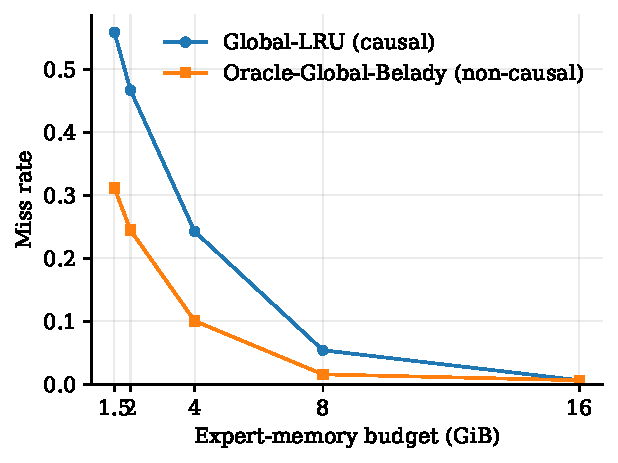
\includegraphics[width=0.72\linewidth]{figures/figure1_miss_rate_vs_budget.pdf}
\caption{Global-LRU (causal) vs.\ Belady comparator $O_B$ (clairvoyant)
miss rate as a function of expert-memory budget (R2-03). Generated by
\texttt{figures/make\_figures.py} from the frozen data snapshot; binary
figure assets were regenerated as presentation artifacts for the
\textsc{AUDIT-ORACLE-001} semantics amendment.}
\label{fig:miss-rate-vs-budget}
\end{figure}

\begin{figure}[t]
\centering
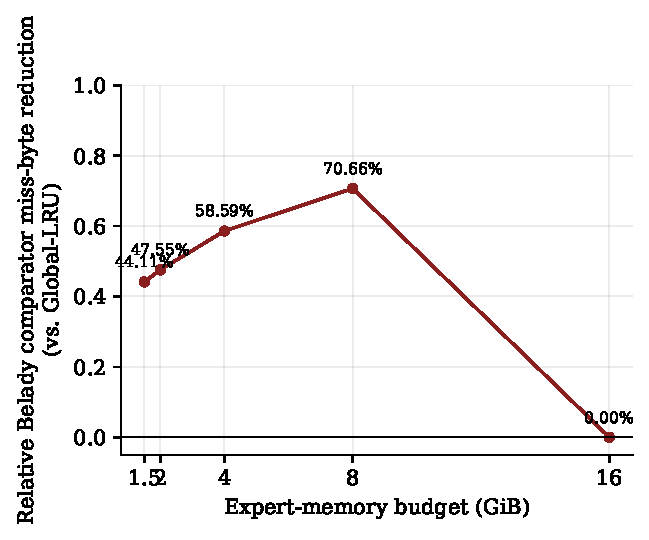
\includegraphics[width=0.72\linewidth]{figures/figure2_relative_headroom_vs_budget.pdf}
\caption{Relative Belady comparator miss-byte reduction over Global-LRU
($G_\budget(\text{Global-LRU},O_B)$, Definition~\ref{def:comparator-gap})
as a function of expert-memory budget (R2-03). The curve rises across the
capacity-constrained points tested ($1.5$--$8$~GiB) and collapses to
zero at $16$~GiB, the first tested budget at which the expert working set
becomes effectively resident. This is a measured comparator gap, not a
proven causal-recovery upper bound.}
\label{fig:headroom-vs-budget}
\end{figure}

\begin{table}[t]
\centering
\caption{Global-LRU vs.\ Oracle-Global-Belady across the tested expert-memory budget sweep (R2-03).}
\label{tab:r2-03-sweep}
\small
\begin{tabular}{@{}rrrrr@{}}
\toprule
Budget (GiB) & Global-LRU misses & Oracle misses & Rel.\ miss-byte reduction & Abs.\ miss-byte reduction (GB) \\
\midrule
1.5 & 81,752 & 45,603 & 44.11\% & 103.57 \\
2 & 68,318 & 35,821 & 47.55\% & 93.42 \\
4 & 35,529 & 14,754 & 58.59\% & 59.86 \\
8 & 7,952 & 2,350 & 70.66\% & 16.18 \\
16 & 973 & 973 & 0.00\% & 0.00 \\
\bottomrule
\end{tabular}
\end{table}


\paragraph{Monotonicity and collapse.} Across the four capacity-constrained
tested points ($1.5$--$8$~GiB, where Global-LRU incurs a nonzero eviction
count), the relative Belady comparator gap rises from $44.11\%$ at
$1.5$~GiB to its largest tested relative value of $70.66\%$ at $8$~GiB.
The largest tested absolute comparator gap among tested points is
$103.57$~GB at $1.5$~GiB. At $16$~GiB, Global-LRU and $O_B$ produce
\emph{identical} miss counts, miss bytes, and zero evictions each: the
expert working set is effectively resident at this budget for the tested
workload, and neither the causal baseline nor the clairvoyant comparator
has evictions to decide. We term $16$~GiB the \emph{first tested
policy-indifference budget}; this is an empirical statement about the
five tested points, not a claim about the mathematically minimal
capacity at which convergence occurs (which may be lower; it was not
swept at finer granularity above $8$~GiB).

\paragraph{Non-monotonic structural gap.} Unlike the comparator gap, the
\emph{structural} Runtime-Sharded-LRU-vs-Global-LRU gap is not monotonic
across the sweep: it is slightly \emph{negative} at $1.5$ and $2$~GiB
(sharding itself reduces miss bytes by $1.82\%$ and $0.39\%$ respectively,
relative to Global-LRU) and positive at $4$ and $8$~GiB ($1.16\%$ and
$2.61\%$). This sign change is a valid observed result
(Section~\ref{sec:recoverable-envelope}) and is not forced to any
particular shape.

\section{Oracle-Bounded Recoverable Envelope (R2-04)}
\label{sec:recoverable-envelope}

R2-04 synthesizes the R2-02/R2-03 evidence into a single decomposition,
applied at every tested budget, and reported here as the headline II-A
result. No new replay, model, or runtime invocation is performed in this
step; it is a pure offline synthesis over already-registered evidence.

\begin{definition}[Structural / information / total decomposition]
\label{def:decomposition}
Let $S$, $G$, $O$ denote the miss-byte totals (at a fixed budget
$\budget$) of Runtime-Sharded-LRU, Global-LRU, and Oracle-Global-Belady
respectively. Define
\begin{align}
\text{Structural sharding gap} &= S - G, \label{eq:structural} \\
\text{Policy-information headroom} &= G - O, \label{eq:information} \\
\text{Total observed upper-bound gap} &= S - O. \label{eq:total}
\end{align}
By construction, Eq.~\eqref{eq:structural} $+$ Eq.~\eqref{eq:information}
$=$ Eq.~\eqref{eq:total} exactly, for both the miss-byte and miss-count
views, independent of the sign of the structural term. The corresponding
\emph{relative} fractions (each normalized by its own comparison's first
operand) are \textbf{not} summed arithmetically, since their denominators
differ -- see Table~\ref{tab:r2-03-sweep} vs.\ the structural
percentages quoted in Section~\ref{sec:sensitivity-capacity}.
\end{definition}

The \emph{policy-information headroom} (Eq.~\ref{eq:information}) is the
quantity of scientific interest for motivating II-B/II-C: it isolates the
cost of imperfect \emph{causal information}, independent of the specific
sharded retention architecture. The \emph{structural sharding gap}
(Eq.~\ref{eq:structural}) is reported for completeness but is not the
focus of this report, and carries the limitation that the offline
Runtime-Sharded-LRU's shard-to-key mapping is statistical rather than the
runtime's exact address-derived mapping.

\begin{table}[t]
\centering
\caption{Headline II-A synthesis (R2-04): oracle-bounded recoverable-envelope summary.}
\label{tab:r2-04-synthesis}
\small
\begin{tabular}{@{}lr@{}}
\toprule
Quantity & Value \\
\midrule
Information headroom at 4~GiB (anchor) & 58.59\% \\
Maximum tested relative information headroom & 70.66\% (at 8~GiB) \\
Maximum tested absolute miss-byte headroom (GB) & 103.57 (at 1.5~GiB) \\
First tested policy-indifference budget (GiB) & 16 \\
Oracle strictly improves at every capacity-constrained point & yes \\
Observed information-headroom curve shape & collapse at effective residency \\
Causally recovered margin & \textsc{not yet measured} (\S~II-C) \\
\bottomrule
\end{tabular}
\end{table}


\paragraph{Absolute vs.\ relative headroom occur at different budgets.}
A single important distinction this synthesis makes explicit: the budget
at which the \emph{relative} information headroom is maximized ($8$~GiB,
$70.66\%$) is \textbf{not} the budget at which the \emph{absolute}
miss-byte headroom is maximized ($1.5$~GiB, $103{,}574{,}900{,}736$
bytes $\approx 103.57$~GB). Under more severe memory pressure (lower
budgets), both Global-LRU and the Oracle incur far more total misses, so
the \emph{absolute} volume of miss bytes the Oracle avoids can be larger
even while its \emph{relative} advantage (as a fraction of Global-LRU's
own, larger, miss-byte total) is smaller. Neither framing is more
``correct''; they answer different engineering questions (fraction of
traffic avoidable vs.\ total bytes avoidable) and are reported
separately, never conflated into one number.

\paragraph{Headroom persistence under pressure.} At every one of the
four capacity-constrained tested budgets ($1.5$--$8$~GiB, where
Global-LRU's own eviction count is nonzero), the Oracle strictly
dominates Global-LRU: a strictly positive miss and miss-byte reduction
is observed at each such point. The $16$~GiB
policy-indifference point is excluded from this statement by definition
(no policy has anything left to decide there, so ``the oracle strictly
improves'' is not a meaningful comparison at that point).

\paragraph{Observed curve shape.} The relative information-headroom
curve (Figure~\ref{fig:headroom-vs-budget}) is classified, deterministically
from the five tested points, as a \emph{rise followed by a collapse at
the observed effective-residency budget}: non-decreasing across
$1.5$--$8$~GiB, then dropping to its global minimum ($0$) exactly at
$16$~GiB, the first tested budget exhibiting policy convergence. This
classification is derived mechanically from the tested points, not
assumed in advance.

\begin{definition}[Future II-C metric -- documented, not evaluated]
\label{def:ii-c-metric}
For a causal baseline with miss bytes $B_\budget$ and a future causal
predictor-driven policy with miss bytes $P_\budget$, both at budget
$\budget$, define
\begin{equation}
\mathrm{FractionOfOracleHeadroomRecovered}_\budget \;=\;
\frac{B_\budget - P_\budget}{B_\budget - O_\budget}, \label{eq:ii-c}
\end{equation}
where $O_\budget$ is the Oracle's miss bytes at that budget. This metric
is defined now, as the scientific bridge from II-A's upper bound to
II-C's demonstrated causal recovery, but \textbf{cannot be evaluated} --
no causal predictor $P$ exists yet. It is reported here purely as a
predeclared target metric for Research II-C.
\end{definition}

\paragraph{Causal recovery: explicitly unmeasured.} We emphasize, as
strongly as the evidence allows: nothing in this section measures or
estimates the fraction of the policy-information headroom that any
practical causal predictor could actually recover. That quantity is
\notyetmeasured{} and is the subject of Research II-C
(Section~\ref{sec:iic-placeholder}), which has not started.

\section{Discussion}
\label{sec:discussion}

\paragraph{What II-A establishes.} Under a validated offline replay
model of a real 30B-A3B MoE coding workload, a substantial gap exists
between causal LRU-family retention and a non-causal Belady-optimal
upper bound, at every tested capacity-constrained expert-memory budget.
This gap -- the policy-information headroom -- is not uniform across
budgets: it is largest, among the tested points, near $8$~GiB in relative
terms and near $1.5$~GiB in absolute terms, and it collapses entirely
once the working set becomes effectively resident (the first tested such
budget being $16$~GiB). The gap persists after decomposing away the
specific cost of the runtime's sharded retention architecture, which is
small and not consistently signed across the sweep.

\paragraph{What II-B establishes.} Under the tested
Qwen3-30B-A3B-Q4\_K\_M protocol, routing is descriptively non-uniform,
sequentially dependent at one-step same-layer resolution, and temporally
local at short horizons relative to a shuffled null. At the same time,
R2-08 shows that cross-workload routing differences exceed temporal drift
under the predeclared comparison (ratio $2.21\times$), with
\texttt{WORKLOAD\_DEPENDENCE\_DOMINANT} as the regime classification.
These results characterize the routing stream; they do not evaluate a
policy.

\paragraph{Observed, inferred motivation, and not established.}
The distinction among these categories is central:
\begin{itemize}
 \item \textbf{Observed:} strong Oracle headroom (II-A); aggregate routing
   concentration, with LFU underperforming Global-LRU at the II-A anchor
   budget; measurable same-layer transition dependence (positive NMI in
   every tested layer); strong short-horizon reuse relative to a shuffled
   null; and cross-workload divergence exceeding temporal drift under the
   deterministic R2-08 protocol.
 \item \textbf{Inference/motivation:} these properties make strictly
   causal working-set prediction scientifically worth testing. The
   short-horizon locality is the most relevant signal for that test; the
   workload dependence implies that a practical predictor may need to be
   robust across workload categories or conditioned on workload context.
 \item \textbf{Not established:} that any causal predictor can recover a
   meaningful fraction of the Oracle-bounded policy-information headroom;
   that prediction accuracy is sufficient; that prefetch, admission, or a
   new retention policy improves runtime; that latency, throughput, or
   memory traffic improves; or that the observed structure generalizes
   across models, quantizations, machines, or non-deterministic decoding
   protocols.
\end{itemize}

\paragraph{Why II-A headroom is not automatically deployable.} An oracle
upper bound requires information no real system has at decision time.
Treating a large oracle gap as an implicit promise of recoverable
performance would conflate an informational upper bound with demonstrated
causal recovery. II-B adds structure, not recovery.

\paragraph{Why II-B structure is not automatically predictive.}
Concentration, transition dependence, reuse locality, and workload
dependence are descriptive properties of observed traces. Each can
motivate a hypothesis about future routing, but none is the same object as
a causal predictor evaluated on future decisions. This is why
Eq.~\eqref{eq:iib-iic-recovery} remains \notyetmeasured{} until
Research~II-C.
\section{Limitations}
\label{sec:limitations}

\subsection*{II-A limitations (preserved, amended for Oracle semantics)}
\begin{itemize}
 \item \textbf{Single validated real workload/trace for II-A.} The II-A
   replay, comparator-gap, sensitivity, and decomposition analyses are
   computed against one captured coding trace (one workload, one
   30B-A3B model instance, one capture budget). Replay fidelity
   (Section~\ref{sec:replay-validation}) is demonstrated for this trace
   only; it is not evidence of fidelity for other workloads, models, or
   capture configurations.
 \item \textbf{Offline replay, not live measurement.} II-A comparisons are
   offline replays against a fixed, already-captured trace. They do not
   measure live runtime behavior under the compared policies themselves.
 \item \textbf{No latency or throughput claim.} Miss bytes are a proxy for
   expert data that would need to be serviced under the replay model. No
   latency, throughput, tokens/second, or SSD-traffic measurement is made
   or implied by II-A or II-B.
 \item \textbf{No causal predictor exists yet.} The Belady comparator gap
   (Section~\ref{sec:recoverable-envelope}) is a measured separation from
   $O_B$, not a demonstrated causal recovery and not a proven bound on
   causal recovery. II-B characterizes routing structure but does not
   evaluate a causal predictor or recover any fraction of that gap.
 \item \textbf{Comparator-objective limitation (\textsc{AUDIT-ORACLE-001},
   CASE~C).} Expert cache objects are $(\ell,e)$ pairs with two byte-size
   classes across layers in the tested trace. The implemented
   \textsc{Oracle-Global-Belady} comparator ($O_B$) uses furthest next use
   only; object byte size does not enter victim ranking. Miss-count and
   miss-byte optimality are not proven under the actual variable-size,
   byte-capacity, multi-key replay semantics. Consequently $B-O_B$ is not
   interpreted as a proven upper or lower bound on causal recovery
   $B-C^*$; $O^* \le O_B$ is known, but $O_B$ and $C^*$ have no guaranteed
   ordering.
 \item \textbf{Statistical, not exact, shard mapping.} The
   Runtime-Sharded-LRU baseline matches the real runtime's \emph{shard
   count} (16 shards at $4$~GiB) but not its exact address-derived
   shard-to-key mapping, which is not reproducible offline.
 \item \textbf{Finite, predeclared budget grid.} The II-A budget sweep
   tests five fixed points ($1.5, 2, 4, 8, 16$~GiB). Behavior between
   tested points and the exact mathematically minimal policy-convergence
   budget are not characterized.
 \item \textbf{LFU auxiliary sweep scope.} The LFU-vs-Global-LRU ranking
   across the R2-03 budget grid is canonical auxiliary R2-03 evidence from
   the same single canonical DEV trace and tested budget grid. It is not
   held-out evaluation and does not establish causal-baseline ordering
   across other workloads, models, or capacities. R2-09A remains necessary.
 \item \textbf{No shard-constrained clairvoyant comparator.} The II-A
   structural and comparator decomposition uses Global-LRU as a shared
   pivot rather than a true sharded-clairvoyant comparison.
\end{itemize}

\subsection*{II-B limitations}
\begin{itemize}
 \item \textbf{Model, quantization, and runtime scope.} II-B evidence is
   limited to Qwen3-30B-A3B-Q4\_K\_M under one consumer-machine runtime
   protocol and one expert-budget configuration context for the tested
   captures. No cross-model, cross-quantization, cross-machine, or
   cross-runtime generalization is measured.
 \item \textbf{Workload scope.} R2-08 tests four workload families
   (coding, reasoning, summarization, instruction), two replicates each.
   The \texttt{WORKLOAD\_DEPENDENCE\_DOMINANT} classification is
   conditional on this tested workload set and protocol.
 \item \textbf{Deterministic decoding protocol.} R2-08 uses
   temperature~$=0.0$, top-$k=1$. Same-workload replicate JSD $=0.0$ is
   therefore interpreted only as reproducibility at the reported
   resolution under deterministic decoding, not as general evidence of
   zero stochastic run-to-run variability.
 \item \textbf{Finite matched horizon.} R2-08 comparisons use matched
   decode horizon $H=388$ with 8 temporal windows of length 48. Longer
   horizons and other windowing choices are not evaluated.
 \item \textbf{Layer-local descriptive analysis.} II-B metrics are
   layer-local and descriptive. No cross-layer primary transition claim is
   made from R2-06, and no causal or mechanistic explanation of routing is
   established.
 \item \textbf{No predictive or runtime evaluation.} II-B includes no
   causal predictor, no predictor accuracy/precision/recall/F1 measurement,
   no prefetch or admission mechanism, no retention-policy replacement, no
   runtime speedup or latency/throughput measurement, and no
   comparator-gap recovery measurement. The comparator-relative metric in
   Eq.~\eqref{eq:iib-iic-recovery} remains \notyetmeasured{}.
 \item \textbf{R2-08 capture-provenance representation.} New R2-08-managed
   capture cells record \texttt{capture\_run\_id}/\texttt{capture\_source}
   as null while preserving trace path, trace SHA, configuration, model
   and runtime SHAs, validation state, and canonical R2-08 run identity.
   This is documented as an intentional representation for internal R2-08
   captures; no capture IDs are invented and no scientific traces are
   modified.
\end{itemize}

\subsection*{DEV/EVAL, EXP-025, and II-C evaluation transparency}
\begin{itemize}
 \item \textbf{DEV characterization evidence.} The canonical R2-01 coding
   trace is documented as a \texttt{dev} split in inspected provenance, and
   the inspected R2-08 workload captures are also documented as
   \texttt{dev}-split characterization captures. Research~II-A and II-B are
   characterization/development tranches, not held-out predictive
   evaluation. Research~II-C's R2-09B contract subsequently froze DEV/EVAL
   roles before any EVAL capture, and R2-10/R2-BRIDGE-01/R2-11/R2-12 each
   captured and sealed their held-out instances before scoring; see
   Section~\ref{sec:iic} for results and Section~\ref{sec:iic-limitations}
   below for this stage's own limitations.
 \item \textbf{EXP-025 applicability.} \textsc{AUDIT-ORACLE-001} classifies
   EXP-025 as a stream/distribution-dependent performance model (P2) whose
   transferability to arbitrary policy-induced miss streams is
   \textsc{UNSUPPORTED} without separate validation. Comparator miss-byte
   reductions must not be converted directly into latency or avoided
   seconds. Future modeled comparisons, if used, must follow
   \begin{equation*}
   \Delta T_{\mathrm{model}} = \mathrm{PerformanceModel}(\mathrm{MissStream}_{B_\mathrm{best}})
   - \mathrm{PerformanceModel}(\mathrm{MissStream}_P)
   \end{equation*}
   with justified scope, and must not be equated with measured end-to-end
   latency, time-to-first answer, or throughput.
 \item \textbf{No numeric practical-effect threshold.} No numeric
   practical-effect threshold is preregistered by this amendment. Any
   future threshold must be derived and frozen in R2-09B using a metric
   justified by the evaluation/performance-model contract.
\end{itemize}

\subsection*{II-C limitations}
\label{sec:iic-limitations}
\begin{itemize}
 \item \textbf{One tested predictive-retention realization.} Only one
   causal predictor (\texttt{decayed\_transition}, decay $0.99$) driving
   one reactive retention-policy realization (\texttt{PredictedProtectPolicy})
   was built and evaluated. Negative results at R2-12 are results about
   this specific realization, not a general statement about predictive
   retention as a design category.
 \item \textbf{Hardware/model/workload scope.} All of R2-09 through R2-12
   were evaluated on one model family (Qwen3-30B-A3B), one consumer host,
   and workload instances drawn from four families (coding, instruction,
   reasoning, summarization). No cross-model, cross-quantization,
   cross-machine, or cross-runtime generalization is claimed.
 \item \textbf{Replay-level benefit does not imply runtime benefit.} R2-11's
   positive replay-level result (\textsc{r2\_11\_pass}) and R2-12's negative
   real-runtime result (\textsc{R2\_12\_FAIL}) are not in tension: they
   measure different quantities (miss bytes per decode step vs. decode
   tokens per second) under different experimental apparatus (offline
   replay vs. the real runtime). Neither bounds the other.
 \item \textbf{Runtime failure does not invalidate predictor quality.} R2-10's
   held-out-confirmed prediction-quality margin (Section~\ref{sec:r2-10})
   is not weakened, retracted, or reclassified by R2-12's negative result.
 \item \textbf{Secondary budgets are not primary decision endpoints.} The
   1.5~GiB and 8~GiB R2-12 budgets are reported descriptively only; neither
   can, under the frozen decision rule, override the primary 4~GiB
   classification, regardless of their own effect sizes or direction.
 \item \textbf{Telemetry gap limits causal attribution at 8~GiB.} The real
   8~GiB canonical records carry no retention-traffic telemetry
   (\texttt{expert\_bytes\_read}/\texttt{expert\_read\_count}/
   \texttt{expert\_miss\_bytes} and every \texttt{expert\_io\_best\_effort}
   sub-field are \texttt{None} for both policies). Any non-retention-overhead
   explanation of the 8~GiB delta is therefore reported as an unverified
   hypothesis, never as a finding.
 \item \textbf{Cross-budget ordering is descriptive.} The ordering of
   measured deltas across 1.5/4/8~GiB (smallest to largest in magnitude) is
   reported as an observation over three tested points, not as evidence of
   a monotonic causal relationship between memory budget and policy
   overhead.
 \item \textbf{Results do not establish universal impossibility.} A negative
   result for one tested reactive-retention realization does not establish
   that no predictive mechanism (e.g., active prefetch, scheduling, or
   compute/I/O overlap -- Section~\ref{sec:iic-related-work}) can convert
   predictive information into real-runtime throughput gain in this problem
   class.
 \item \textbf{Host/environment constraints are exactly those frozen in the
   protocol, no more.} R2-12's machine-state and readiness gates
   (AC power, operator-attested clean environment, thermal cooldown policy,
   power mode) are exactly the conditions frozen in
   \texttt{machine\_state\_contract.json} and \texttt{execution\_plan.json}
   before acquisition. No condition not formally frozen there (e.g., a
   specific battery-percentage or ambient-temperature threshold used
   elsewhere in the Argine programme) is retroactively applied as an
   exclusion criterion to R2-12's evidence.
 \item \textbf{Runtime conformance was reached iteratively.} The runtime
   binary realizing the retention-policy integration for R2-12 required
   several realization/conformance iterations before reaching an accepted
   conformance state; it is not byte-identical to the R2-01 validated
   replay-comparison runtime. This is disclosed rather than assumed from a
   single attempt.
\end{itemize}

\section{Routing Characterization}
\label{sec:iib}

The clairvoyant-comparator-gap analysis measured a substantial miss-byte gap between Global-LRU
and the implemented clairvoyant Belady-style comparator $O_B$ under
constrained memory (Sections~\ref{sec:oracle-headroom}--\ref{sec:recoverable-envelope}).
After \textsc{AUDIT-ORACLE-001}, that comparator gap is not interpreted as a
proven byte-optimal bound or a proven upper bound on causal recovery; it
shows separation from a non-causal comparator, not whether a causal policy
can close it. This section asks the necessary prior question:

\begin{quote}
\emph{Is MoE expert routing sufficiently structured, local, and
workload-dependent to justify attempting causal working-set prediction?}
\end{quote}

This is a descriptive characterization stage. It does \emph{not}
answer whether a predictor works, whether prefetch improves runtime,
whether a new retention policy reduces the measured clairvoyant-comparator
gap or improves on selected causal baselines, whether inference
becomes faster, or whether the result generalizes across models. Those
questions belong to the causal-prediction and real-runtime validation
stage or later work.

\subsection{Evidence Base and Scope}
\label{sec:iib-scope}

Table~\ref{tab:iib-map} lists the four canonical PASS experiments.
R-05--R-07 are offline analyses over the same validated R-01 coding
trace used throughout the clairvoyant-comparator-gap analysis
(the canonical trace identified by H-TRACE-R01; Appendix~\ref{sec:hash-registry}),
with layer-local expert identity, no new model/runtime invocation, and no
new trace capture. R-08 adds controlled captures for four workload
families (coding, reasoning, summarization, instruction), two replicates
each, under a fixed Qwen3-30B-A3B-Q4\_K\_M / 4~GiB expert-budget
consumer-machine protocol with deterministic decoding
(temperature~$=0.0$, top-$k=1$). One \code{coding-v1/seed-42} cell reuses the
canonical R-01 trace; seven cells were newly captured for R-08. All
analysis is layer-local and descriptive.

\begin{table}[t]
\centering
\caption{Routing-characterization experiment map (canonical PASS evidence only).}
\label{tab:iib-map}
\small
\begin{tabularx}{\linewidth}{@{}l >{\raggedright\arraybackslash}p{2.9cm}
  >{\raggedright\arraybackslash}X l l@{}}
\toprule
Exp. & Question & Primary metrics & Run & Outcome \\
\midrule
R-05 & Expert frequency and concentration & normalized entropy, effective experts, top-8 share, 80\% mass & \texttt{da82e15b61c9\ldots} & PASS \\
R-06 & Routing transition structure & same-layer NMI, conditional entropy, self-transition lift & \texttt{2e075161f024\ldots} & PASS \\
R-07 & Reuse distance and working-set structure & reuse fractions, gaps, distinct-intervening distance, working set, shuffled null & \texttt{af28e8c6dc50\ldots} & PASS \\
R-08 & Routing drift and workload dependence & temporal/replicate/cross-workload JSD, top-8 Jaccard distance, regime & \texttt{6165471a1257\ldots} & PASS \\
\bottomrule
\end{tabularx}
\end{table}


\paragraph{R-08 capture-provenance audit.}
In the canonical R-08 capture matrix, the reused
\code{coding-v1/seed-42} cell records the run identifier and capture
source of the upstream R-01 capture, while the seven
R-08-managed new captures carry a null run identifier and a null capture
source. This is treated as an intentional
provenance representation of R-08-internal captures, not as a missing
scientific trace: every canonical cell records a trace path, trace
digest, workload identity, seed, model digest, runtime digest,
configuration fingerprint, validation state, and canonical status, all
bound to the canonical R-08 run and its canonical digest
(H-R08-CANONICAL; Appendix~\ref{sec:hash-registry}).
The paper freeze does not invent capture IDs and does not modify
scientific traces.

\subsection{R-05: Expert Frequency and Concentration}
\label{sec:r2-05}

R-05 measures aggregate layer-local routing frequency on the validated
trace. Table~\ref{tab:r2-05-summary} and Figure~\ref{fig:b1-concentration}
summarize the result.

\begin{table}[t]
\centering
\caption{R2-05 expert frequency and concentration summary (descriptive, layer-local).}
\label{tab:r2-05-summary}
\small
\begin{tabular}{@{}lr@{}}
\toprule
Quantity & Value \\
\midrule
Total routing requests (token-expert assignments) & 205,048 \\
Layers / nominal experts per layer / top-$k$ & 48 / 128 / 8 \\
Median normalized entropy & 0.8522 \\
Median effective expert fraction & 0.5136 \\
Median effective experts ($\approx$) & 65.7 / 128 \\
Median top-8 traffic share & 0.3001 \\
Top-8 share range (min--max) & 0.1595--0.4074 \\
Median experts for 80\% traffic & 43 \\
80\% mass range (min--max experts) & 31--68 \\
Most / least concentrated layer & 31 / 0 \\
\bottomrule
\end{tabular}
\end{table}


\begin{figure}[t]
\centering
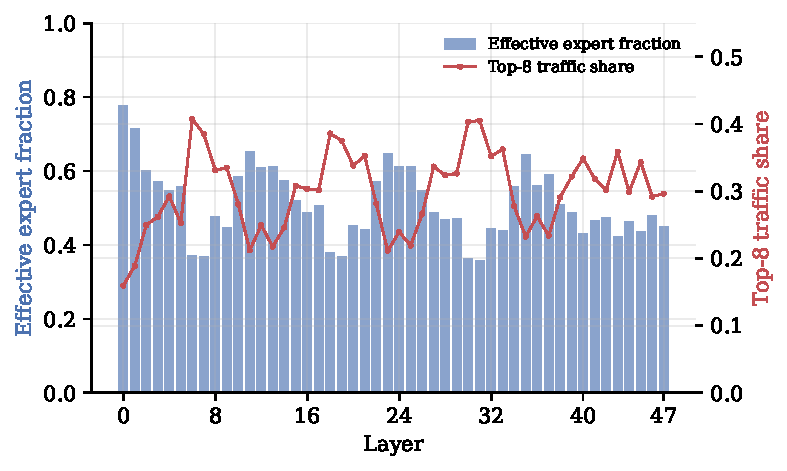
\includegraphics[width=0.78\linewidth]{figures/figure_b1_r2_05_concentration.pdf}
\caption{Layer-wise R-05 routing concentration on the validated coding
trace. Bars show effective expert fraction (effective experts divided by
128 nominal experts); the line shows top-8 traffic share per layer. The
figure measures aggregate non-uniformity across layers, not temporal
stability and not cache performance.}
\label{fig:b1-concentration}
\end{figure}

Across 205,048 token-expert assignment observations, routing is strongly
non-uniform at the aggregate level: the median effective expert fraction
is $0.514$ (about $65.7$ of $128$ nominal experts), the median top-8
traffic share is $0.300$, and the median number of experts required for
80\% of traffic is $43$ (range $31$--$68$).

This concentration does not imply that static frequency-based LFU is a
sufficient retention policy in the tested pressure regime. R-03's
canonical auxiliary evidence shows that static LFU incurs more miss bytes
than Global-LRU at every tested capacity-constrained budget from 1.5 to
8~GiB on the same DEV trace, tying at 16~GiB
(Table~\ref{tab:r2-03-lfu-aux}). Thus substantial aggregate frequency
concentration exists, but static frequency-based LFU does not outperform
recency-based Global-LRU anywhere in the tested pressure regime on this
trace and budget grid. This motivates examining temporal and sequential
information beyond aggregate frequency. R-06 and R-07 test complementary
sequential and temporal structure.

\subsection{R-06: Routing Transition Structure}
\label{sec:r2-06}

R-06 asks whether the previous same-layer routing state carries
information about the next same-layer routing state beyond marginal
frequency. The unit is a \emph{pairwise set-to-set transition
observation}: for consecutive token selections in a layer, every expert in
the source top-8 selection is paired with every expert in the target
top-8 selection. The resulting 1,637,312 observations are therefore
pairwise transition observations generated by top-8 $\times$ top-8
relationships; they are \emph{not} 1.64~million independent samples.

\begin{table}[t]
\centering
\caption{R2-06 routing transition structure summary (same-layer, pairwise set-to-set observations).}
\label{tab:r2-06-summary}
\small
\begin{tabular}{@{}lr@{}}
\toprule
Quantity & Value \\
\midrule
Pairwise set-to-set transition observations & 1,637,312 \\
Layers / nominal experts per layer & 48 / 128 \\
Median same-layer NMI & 0.0989 \\
NMI range (min--max) & 0.0826--0.1368 \\
Layers with positive NMI & 1.00 \\
Median conditional entropy & 3.7353 \\
Median self-transition lift & 4.1850 \\
Median top-1 outgoing probability & 0.0904 \\
Median outgoing effective-target fraction & 0.7170 \\
Maximum supported transition lift (layer) & 31.90 (L37) \\
Strongest / weakest NMI layer & 37 / 45 \\
\bottomrule
\end{tabular}
\end{table}


\begin{figure}[t]
\centering
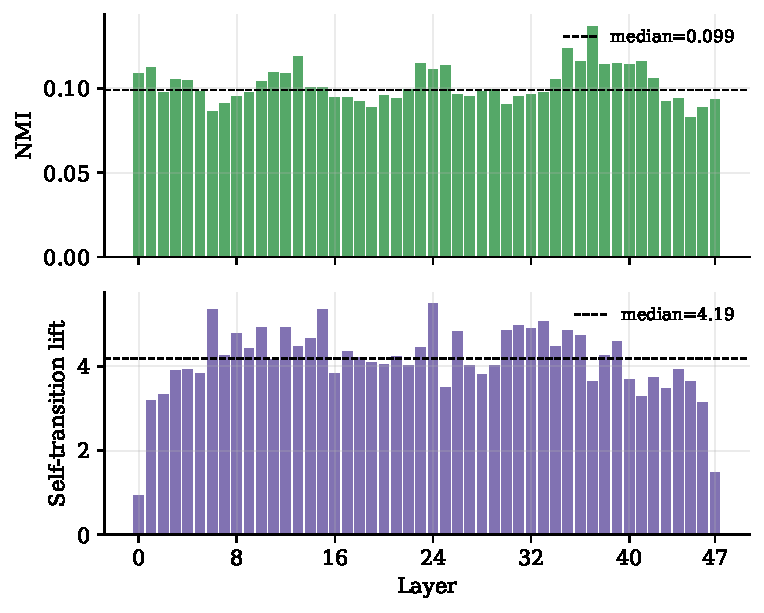
\includegraphics[width=0.78\linewidth]{figures/figure_b2_r2_06_transitions.pdf}
\caption{R-06 same-layer transition structure by layer. Top: normalized
mutual information (NMI) between consecutive token-to-token expert
selections. Bottom: median self-transition lift. Dashed lines mark medians
across layers. NMI measures measurable dependence, not predictor accuracy.}
\label{fig:b2-transitions}
\end{figure}

Table~\ref{tab:r2-06-summary} and Figure~\ref{fig:b2-transitions} show
measurable sequential dependence in every tested layer (fraction with
positive NMI $=1.0$). Median NMI is $0.099$ (range $0.083$--$0.137$),
with median conditional entropy $3.735$. This means the previous routing
state provides a measurable reduction in uncertainty about the next
routing state at the measured resolution. NMI is not translated into
prediction accuracy, and R-06 does not train or evaluate a predictor.

\subsection{R-07: Reuse Distance and Working-Set Structure}
\label{sec:r2-07}

R-07 measures layer-local reuse distance and working-set growth, and
compares observed routing to a deterministic shuffled null that preserves
marginals while destroying temporal order. Table~\ref{tab:r2-07-summary}
and Figure~\ref{fig:b3-reuse} summarize the result.

\begin{table}[t]
\centering
\caption{R-07 reuse distance and working-set summary (observed vs deterministic shuffled null).}
\label{tab:r2-07-summary}
\small
\begin{tabular}{@{}lr@{}}
\toprule
Quantity & Value \\
\midrule
Reuse events / first observations & 199,784 / 5,264 \\
Median immediate reuse (gap=1) & 0.4256 \\
Median reuse $\le 4$ / $\le 16$ positions & 0.6415 / 0.8602 \\
Median token reuse gap / p90 gap & 2 / 24 \\
Median distinct-intervening reuse distance & 8 \\
Median working set $W_8/W_{32}/W_{128}/W_{256}$ & 30.0/57.0/89.5/102.5 \\
Frequency--reuse-gap Spearman (descriptive) & -0.6506 \\
Immediate reuse: observed / null / ratio & 0.4256 / 0.1873 / 2.27$\times$ \\
Reuse $\le 4$: observed / null / ratio & 0.6415 / 0.4780 / 1.34$\times$ \\
Reuse $\le 16$: observed / null / ratio & 0.8602 / 0.8208 / 1.05$\times$ \\
Median gap: observed / null & 2 / 5 \\
Distinct-intervening: observed / null & 8 / 24 \\
\bottomrule
\end{tabular}
\end{table}


\begin{figure}[t]
\centering
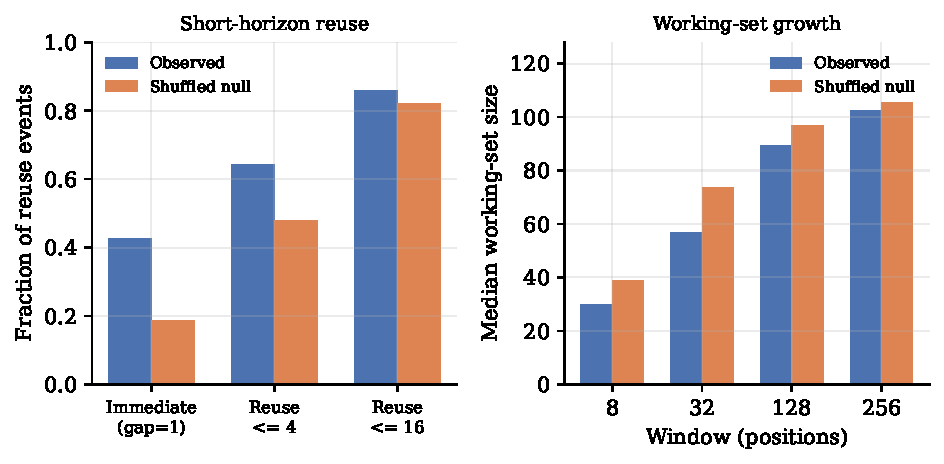
\includegraphics[width=0.92\linewidth]{figures/figure_b3_r2_07_reuse_locality.pdf}
\caption{R-07 observed routing locality versus a deterministic shuffled
null. Left: fraction of reuse events at immediate, $\leq 4$, and
$\leq 16$ position horizons. Right: median working-set size at windows
$W_8, W_{32}, W_{128}, W_{256}$. The departure from the null is strongest
at short horizons, consistent with temporally local structure.}
\label{fig:b3-reuse}
\end{figure}

Observed reuse is concentrated at short horizons. Immediate reuse is
$0.426$ versus $0.187$ for the shuffled null ($2.27\times$); reuse within
4 positions is $0.642$ versus $0.478$; reuse within 16 positions is
$0.860$ versus $0.821$. The observed median token reuse gap is $2$
(null $5$), and the observed median distinct-intervening reuse distance is
$8$ (null $24$). Working sets are smaller than the null at short and
medium windows ($W_8$: $30$ vs.\ $39$; $W_{32}$: $57$ vs.\ $73.5$;
$W_{128}$: $89.5$ vs.\ $97$; $W_{256}$: $102.5$ vs.\ $105.5$).

The strongest departure from the null occurs at short horizons and
narrows at longer horizons. This is a descriptive locality result, not a
prediction result. It motivates short-horizon causal prediction as the
scientifically relevant next test.

\subsection{R-08: Routing Drift and Workload Dependence}
\label{sec:r2-08}

R-08 tests whether routing structure is stable within a workload over
time, reproducible under the same workload and protocol, and dependent on
workload category. The canonical matrix has four workloads
(\texttt{coding-v1}, \texttt{reasoning-v1}, \texttt{summarization-v1},
\texttt{instruction-v1}) with two replicates each, all valid, using the
same model SHA, runtime SHA, and compatible configuration fingerprints.
Comparisons use a matched decode horizon $H=388$ and 8 temporal windows of
length 48.

\begin{table}[t]
\centering
\caption{R2-08 routing drift and workload-dependence scale comparison.}
\label{tab:r2-08-summary}
\small
\begin{tabular}{@{}lr@{}}
\toprule
Quantity & Value \\
\midrule
Matrix & 4 workloads $\times$ 2 replicates = 8 cells \\
Reused / new captures & 1 / 7 \\
Matched decode horizon $H$ & 388 \\
Temporal windows / window length & 8 / 48 \\
Median temporal JSD & 0.135556 \\
Median same-workload replicate JSD & 0.0\,\footnotemark[1] \\
Median cross-workload JSD & 0.299496 \\
Cross-workload / temporal ratio & 2.2094$\times$ \\
Median top-8 temporal Jaccard distance & 0.606061 \\
Predeclared regime & WORKLOAD\_DEPENDENCE\_DOMINANT \\
Most / least stable workload & instruction-v1 / coding-v1 \\
Most / least stable layer & 47 / 12 \\
Strongest workload pair (median layer JSD) & reasoning-v1 (s42) vs instruction-v1 (s42), 0.421342 \\
Configuration compatibility & true \\
\bottomrule
\end{tabular}
\vspace{2pt}
\par\footnotesize\textsuperscript{1}Under the deterministic decoding protocol (temperature~$=0.0$, top-$k=1$); interpreted as a reproducibility check at the reported resolution, not as a general claim of zero stochastic run-to-run variability.
\end{table}


\begin{figure}[t]
\centering
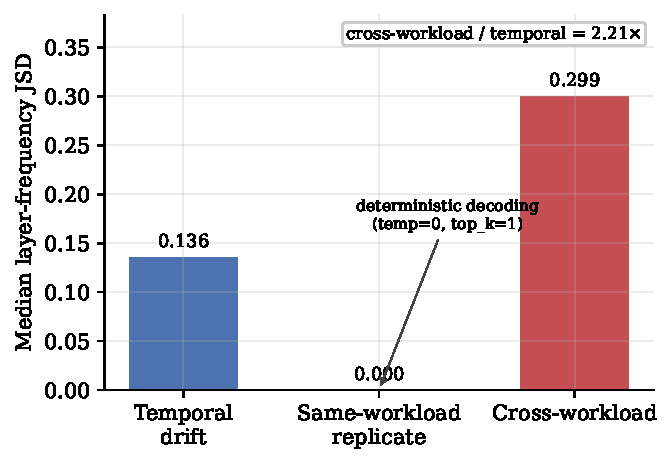
\includegraphics[width=0.68\linewidth]{figures/figure_b4_r2_08_scale_comparison.pdf}
\caption{R-08 scale comparison of median layer-frequency Jensen--Shannon
divergence (JSD): temporal drift within captures, same-workload replicate
divergence, and cross-workload divergence. The same-workload replicate bar
is $0.000$ under the deterministic decoding protocol (temperature~$=0.0$,
top-$k=1$) at the reported resolution; it is a reproducibility check, not
a general claim of zero stochastic variability.}
\label{fig:b4-scale}
\end{figure}

Table~\ref{tab:r2-08-summary} and Figure~\ref{fig:b4-scale} show that
cross-workload divergence dominates the predeclared comparison. Median
cross-workload JSD is $0.299$, median temporal JSD is $0.136$, and the
cross-workload/temporal ratio is $2.21\times$ (predeclared dominance
threshold $1.5\times$). The strongest tested workload pair is
\texttt{reasoning-v1} seed~42 versus \texttt{instruction-v1} seed~42
(median layer frequency JSD $0.421$). The predeclared regime is
\texttt{WORKLOAD\_DEPENDENCE\_DOMINANT}.

Under the deterministic decoding protocol, median same-workload replicate
JSD is $0.0$ at the reported resolution. This must be interpreted
narrowly: \emph{under the deterministic decoding protocol used here,
same-workload replicate frequency distributions were identical at the
reported resolution}. It is a reproducibility check, not evidence that
run-to-run stochastic variability is zero in general. The result
strengthens attribution of the observed differences to temporal position
and workload category within this protocol; it does not generalize beyond
this protocol.

\subsection{Synthesis and Connection to Causal Prediction}
\label{sec:iib-synthesis}

This evidence forms a constrained chain. R-05 shows that routing is
non-uniform, while canonical auxiliary R-03 evidence shows that static
LFU does not outperform Global-LRU at any tested capacity-constrained
point on the DEV trace (tying only at 16~GiB effective residency). R-06
shows that previous routing state carries measurable information about
subsequent routing. R-07 shows that this structure is
strongest at short horizons, with reuse and working sets more compact than
a shuffled null. R-08 shows that the routing signature varies materially
by workload under the tested protocol.

The central restrained claim is therefore:

\begin{quote}
\emph{Under the tested Qwen3-30B-A3B-Q4\_K\_M workload and runtime
protocol, expert routing exhibits substantial aggregate concentration,
measurable transition dependence, strong short-horizon reuse locality, and
pronounced workload dependence. These properties establish empirical
structure that can motivate causal working-set prediction, but do not
themselves demonstrate predictive accuracy or runtime improvement.}
\end{quote}

This characterization connects to the earlier analysis through the measured
clairvoyant-comparator gap, which measures the separation between a simple
causal baseline and the implemented comparator $O_B$; here we assess whether
observable routing history contains structure that could, in principle,
allow a stronger causal policy to reduce part of that measured gap.
The causal-prediction and real-runtime validation stage defines the signed
comparator-relative recovery metric
\begin{equation}
\label{eq:comparator-relative-recovery}
\mathrm{RecoveryOfBeladyGap}
  = \frac{B - P}{B - O_B},
\end{equation}
where $B$ is selected causal baseline miss bytes, $P$ is predictor-driven
miss bytes, and $O_B$ is implemented comparator miss bytes, all at fixed
budget and workload. The metric is signed; values $>1$ are possible under
CASE~C and mean $P$ beats $O_B$, not $O^*$. This metric is not populated
by the routing characterization, and the actual reported evaluation
(Section~\ref{sec:iic}) instead reports its predictor's performance via the
R-09B/R-10 held-out recall$@k$ margin and its retention policy's
performance via the frozen R-11/R-12 metrics
(miss bytes per decode step and decode tokens per second respectively),
which are the
metrics the frozen decision rules for that stage actually define and
apply; this equation is retained here as the originally-planned
connective metric between the earlier analyses and the causal-prediction
stage, not as a value that was ultimately computed and reported.
\section{Research II-C -- Causal Prediction, Replay Retention, and Real-Runtime Validation}
\label{sec:iic}

Research~II-C evaluates whether a strictly causal predictor can exploit the
routing structure characterized in Research~II-B, whether a predictor-driven
retention policy built on it improves a replay-level retention metric, and
whether that replay-level improvement converts into measured real-runtime
decode-throughput improvement. We preserve throughout this section the
three-level distinction stated in the programme's original roadmap
(Section~\ref{sec:introduction}'s enumeration of II-A/II-B/II-C, and
Section~\ref{sec:recoverable-envelope}'s unmeasured-comparator-relative
discussion, both retained unchanged): \emph{prediction} (R2-09/R2-10),
\emph{replay-level retention} (R2-BRIDGE-01/R2-11), and \emph{real runtime}
(R2-12) are three separate, differently-scoped measurements. A result at one level does not imply, and
is not treated here as implying, the same result at another level.

\begin{table}[t]
\centering
\caption{Causal-prediction and real-runtime-validation milestone summary.}
\label{tab:c1-milestones}
\small
\begin{tabular}{@{}lp{6.3cm}l@{}}
\toprule
Milestone & Purpose & Closure state \\
\midrule
R-09A/B & Freeze benchmark contract; DEV causal-baseline tournament & CLOSED \\
R-10 & Held-out EVAL of selected predictor (decayed\_transition) & CLOSED / Category B supported \\
R-BRIDGE-01 & Prospective replay retention feasibility check & CLOSED / BRIDGE\_POSITIVE \\
R-11 & Confirmatory replay retention evaluation, 72 cells & CLOSED / R2\_11\_PASS \\
R-12 & Real-runtime validation, 1.5/4/8 GiB & CLOSED / R2\_12\_FAIL (primary) \\
\bottomrule
\end{tabular}
\end{table}


\subsection{R2-09/R2-10 -- Causal Working-Set Prediction}
\label{sec:r2-10}

Under the frozen R2-09B benchmark contract (DEV/EVAL role separation,
leakage-safe baseline selection, deterministic double-scoring), the DEV
causal-baseline tournament selected \texttt{decayed\_transition} (decay
$=0.99$) as the best-performing causal predictor family on 8 DEV cells,
with DEV $h=1$ mean recall$@k$ $0.439397$ against the best trivial causal
baseline (\texttt{last\_observation}, $0.406808$), an absolute margin of
$0.032589$. Under \texttt{decision\_rules.json}'s DEV-anchored category
definitions this margin is classified Category~B
(\textsc{measurable\_improvement\_insufficient\_for\_retention}): measurable
and consistent across all 8 DEV cells and all 4 workload families, but not
large enough to meet the Category~C bar on its own.

On 4 sealed, held-out EVAL instances (captured and sealed before scoring),
the selected predictor's $h=1$ mean recall$@k$ was $0.449817$, exceeding its
own DEV figure (no sign of DEV overfitting), and beating both trivial
baselines: \texttt{last\_observation} ($0.401473$, $+12.04\%$ relative) and
\texttt{global\_frequency} ($0.349480$, $+28.71\%$ relative). The margin over
\texttt{last\_observation} was positive in all 4 workloads at every tested
horizon ($h=1,4,16$); the margin over \texttt{global\_frequency} was positive
in all 4 workloads at $h=1$ and $h=4$ but negative in one workload
(instruction-eval-v1) at $h=16$, which we report as a disclosed negative
finding rather than omit. Because \texttt{decision\_rules.json}'s Category
A/B/C criteria are textually anchored to the DEV corpus, this held-out
evidence \emph{supports, without promoting}, the DEV-based Category~B
classification: EVAL data cannot itself satisfy a category defined only over
DEV cells. R2-09/R2-10 therefore establish a measurable, held-out-confirmed
causal prediction margin over trivial baselines, at a magnitude the frozen
rules themselves judge insufficient, standing alone, to justify retention
integration.

\begin{table}[t]
\centering
\caption{R2-09/R2-10 held-out EVAL mean recall@k by horizon (4 held-out instances, equal weight).}
\label{tab:c2-predictor}
\small
\begin{tabular}{@{}lccc@{}}
\toprule
Predictor & $h{=}1$ & $h{=}4$ & $h{=}16$ \\
\midrule
decayed\_transition (selected) & 0.4498 & 0.3611 & 0.3403 \\
last\_observation & 0.4015 & 0.2995 & 0.2648 \\
global\_frequency & 0.3495 & 0.3429 & 0.3322 \\
\bottomrule
\end{tabular}
\end{table}


\begin{figure}[t]
\centering
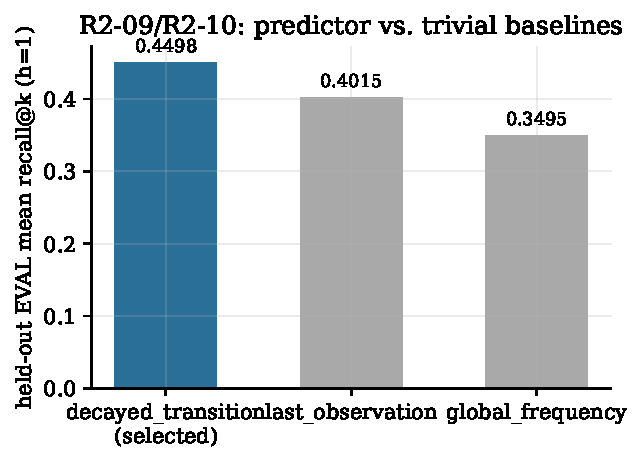
\includegraphics[width=0.68\linewidth]{figures/figure_c1_r2_10_predictor_comparison.pdf}
\caption{R2-09/R2-10: held-out EVAL mean recall@k ($h{=}1$) for the
selected predictor vs.\ both trivial causal baselines. Values read from
Table~\ref{tab:c2-predictor}.}
\label{fig:c1-predictor}
\end{figure}

\subsection{R2-BRIDGE-01 -- Retention Feasibility Bridge}
\label{sec:bridge01}

The literal historical statement that \emph{``R2-11 was NOT PROPOSED under
the original frozen R2-10 decision rules''} remains true and unchanged: the
Category~B finding above does not, by the original rule's own text, provide
a path to proposing a retention-integration experiment. R2-BRIDGE-01 is a
separate, later-frozen, prospective protocol -- not a retroactive
reinterpretation of R2-10's rule -- whose purpose was precisely to determine
whether \emph{new} evidence could justify proposing such an experiment.

Under a frozen contract and a DEV-selection rule fixed before held-out
capture, R2-BRIDGE-01 wired the selected R2-10 predictor into a reactive
retention policy, \texttt{PredictedProtectPolicy}, and compared it against
the aged-frequency baseline \texttt{B\_selected(M)} on 4 fresh held-out
instances, using \texttt{miss\_bytes\_per\_decode\_step} in replay. At the
primary 4~GiB budget, \texttt{PredictedProtect} reduced mean miss bytes per
decode step by $57{,}784.861$ (relative $-0.023084\%$) relative to
\texttt{B\_selected(M)}, with every one of the 4 held-out workloads
individually non-positive. At the two secondary budgets tested, the effect
was also non-positive (1.5~GiB: $-0.1335\%$; 8~GiB: exactly $0.0\%$, an exact
tie). R2-BRIDGE-01 was classified \textsc{bridge\_positive}: the effect is
small in absolute terms, but it is consistently signed across all tested
workloads and budgets, and that consistency -- not its magnitude -- is what
the frozen rule treats as sufficient to justify \emph{proposing} a new,
separate R2-11 protocol prospectively. This does not rewrite, and is not
read here as rewriting, the historical R2-10-rule statement above; both
statements hold simultaneously. No runtime-speedup claim is made or implied
by R2-BRIDGE-01: the metric is a replay-level memory-traffic proxy, not a
timing measurement.

\begin{figure}[t]
\centering
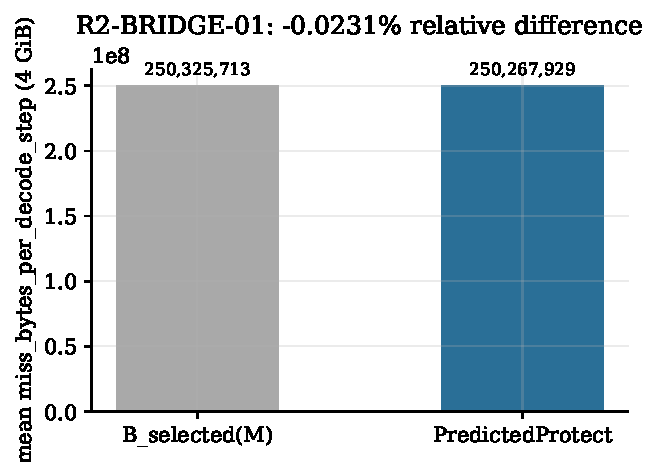
\includegraphics[width=0.6\linewidth]{figures/figure_c2_r2_bridge01_miss_bytes.pdf}
\caption{R2-BRIDGE-01: mean miss\_bytes\_per\_decode\_step, B\_selected(M)
vs.\ PredictedProtect, primary 4~GiB budget, 4 held-out instances.}
\label{fig:c2-bridge}
\end{figure}

\subsection{R2-11 -- Confirmatory Replay-Level Retention Evaluation}
\label{sec:r2-11}

R2-11 is the confirmatory evaluation proposed on the strength of
R2-BRIDGE-01's prospective result, run under its own frozen Phase-0 protocol
(fixed before any capture). It compares \texttt{PredictedProtect} against
\texttt{B\_selected(M)} on 12 fresh workload instances $\times$ 3 budgets
(1.5/4/8~GiB) $\times$ 2 policies, a $72$-cell design; all 72 cells were
computed, with 0 failures and 0 budget-constraint violations across the
full design.

At the frozen primary 4~GiB budget, the mean paired delta in
\texttt{miss\_bytes\_per\_decode\_step} was $-87{,}476.85$
(\texttt{PredictedProtect} minus \texttt{B\_selected(M)}), with a paired
bootstrap 95\% confidence interval of $[-154{,}123.32,\,-27{,}178.93]$ (100{,}000
resamples, fixed seed, independently audited for determinism) --
entirely below zero. 9 of the 12 workload instances individually improved
($\le 0$). At the 1.5~GiB stress budget the effect was larger in magnitude
($-779{,}296.06$); at the 8~GiB budget the effect was an exact tie
($0.0$ for all 12 workload instances), consistent with the budget being
generous enough, on these workloads, that eviction pressure -- and hence any
opportunity for a predictive eviction policy to change which object is
evicted -- is minimal or absent. R2-11's frozen decision rule classifies
this primary-budget result \textsc{r2\_11\_pass}.

We state explicitly, as the programme's evidence-level distinction requires:
\textsc{r2\_11\_pass} is a statement about
\texttt{miss\_bytes\_per\_decode\_step} under offline replay. It is
\emph{not} a runtime, latency, or throughput measurement, and it does not by
itself establish that any real decode-time benefit follows. That question is
R2-12's.

\begin{table}[t]
\centering
\caption{Replay-level retention results: mean paired delta in miss\_bytes\_per\_decode\_step (PredictedProtect $-$ B\_selected(M)).}
\label{tab:c3-retention}
\small
\begin{tabular}{@{}llrrrl@{}}
\toprule
Stage & Budget & $\Delta$ (bytes/step) & Relative & 95\% CI & Status \\
\midrule
R2-BRIDGE-01 (prospective) & 4 GiB (primary) & -57,784.86 & -0.0231\% & --- & BRIDGE\_POSITIVE \\
R2-11 (confirmatory) & 1.5 GiB (stress) & -779,296.06 & --- & --- & descriptive \\
R2-11 (confirmatory) & 4 GiB (primary) & -87,476.85 & --- & [-154,123.32, -27,178.93] & R2\_11\_PASS \\
R2-11 (confirmatory) & 8 GiB (null-control) & 0.00 & 0.0000\% & --- & exact tie \\
\bottomrule
\end{tabular}
\end{table}


\begin{figure}[t]
\centering
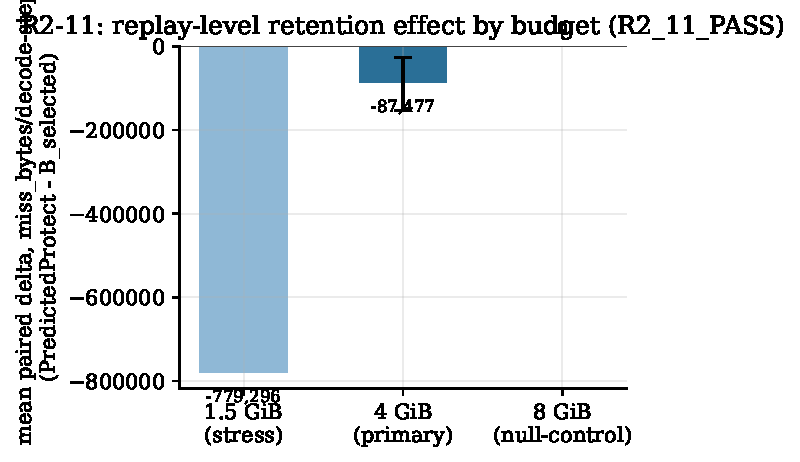
\includegraphics[width=0.78\linewidth]{figures/figure_c3_r2_11_replay_effect.pdf}
\caption{R2-11: mean paired delta in miss\_bytes\_per\_decode\_step by
budget (PredictedProtect $-$ B\_selected(M)); error bar shows the frozen
primary-budget 95\% paired bootstrap CI. 1.5/8~GiB are shown for context
and do not carry an independent R2-12-style classification at this stage.}
\label{fig:c3-r2-11}
\end{figure}

\subsection{R2-12 -- Real-Runtime Validation}
\label{sec:r2-12}

R2-12 tests whether R2-11's replay-level retention improvement converts into
measured real-runtime decode-throughput improvement, using the actual
30B-class runtime (not offline replay), under a frozen Phase-0 protocol with
machine-state and readiness gates fixed before any canonical acquisition.
Realizing the retention-policy integration in the real runtime required
several iterations before reaching an accepted conformance state (the
runtime binary used here is not byte-identical to the R2-01 validated
replay-comparison runtime; conformance was reached only after repeated
realization/repair cycles, not on the first attempt -- see
Section~\ref{sec:iic-limitations}). The frozen primary endpoint is the
4~GiB budget; 1.5~GiB (``stress'') and 8~GiB (``null-control'') are
secondary, descriptive budgets that cannot override the primary
classification under the frozen decision rule.

Across all three budgets, $144/144$ physical canonical launches were
completed (48 each at 1.5/4/8~GiB; 40 counted and 8 warmup per budget),
with all per-budget output-equivalence and integrity checks passing and the
frozen contract digest unchanged throughout. One latent software defect was
found and fixed mid-campaign -- the primary-analysis loader lacked a
budget-scoping filter, which was harmless until multiple budgets' canonical
records coexisted on disk -- and is disclosed here rather than silently
corrected; its fix is covered by a dedicated mixed-budget contamination
regression test, and the previously-committed 4~GiB result was verified
byte-identical before and after the fix.

At the \textbf{primary 4~GiB budget}, the observed mean paired delta in
decode tokens-per-second was $\mathbf{-0.171721}$
(\texttt{PredictedProtect} minus \texttt{B\_selected(M)}), 95\% paired
bootstrap CI $[-0.259917,\,-0.091642]$, entirely at or below zero;
\texttt{B\_selected(M)} won 18 of 20 counted pairs. Per the frozen primary
decision rule, this is sufficient on its own for a negative classification;
the separate overhead-dominance clause need not be evaluated. \textbf{R2-12's
primary classification is \textsc{r2\_12\_fail}.}

At the \textbf{1.5~GiB stress budget} (descriptive only, no independent
classification), the observed delta was $-0.068831$ TPS ($-2.9238\%$), 95\%
CI $[-0.093256,\,-0.054608]$. At the \textbf{8~GiB null-control budget}
(descriptive only), the observed delta was $-0.4373259$ TPS ($-6.5166\%$),
95\% CI $[-0.531584,\,-0.366601]$, with \texttt{B\_selected(M)} winning all
20 counted pairs. R2-11 found an exact replay-level retention tie at
8~GiB; R2-12 does not assume runtime equality follows from that tie, and
treats 8~GiB as a useful null/control condition in exactly this sense: a
material real-runtime difference despite (replay-level) retention-traffic
parity would, if it could be attributed to a specific mechanism, point away
from retention and toward some other overhead source. However, the real
8~GiB canonical records carry \emph{no} retention-traffic telemetry for
either policy at this budget (\texttt{expert\_bytes\_read},
\texttt{expert\_read\_count}, \texttt{expert\_miss\_bytes}, and every
\texttt{expert\_io\_best\_effort} sub-field are \texttt{None} in the real
acquisition for both policies). Consequently, any explanation of the 8~GiB
delta in terms of non-retention (e.g., prediction-policy bookkeeping)
overhead remains an explicitly unverified \emph{hypothesis}, not a
finding, in this manuscript.

Descriptively, the magnitude of the measured delta is smallest at 1.5~GiB
($-2.92\%$), intermediate at 4~GiB ($-4.77\%$), and largest at 8~GiB
($-6.52\%$). We state this as an \emph{observation over three tested
points}, not as evidence of a monotonic causal relationship between memory
budget and policy overhead, a claim the available design cannot support
with only three budget points and no isolated overhead mechanism.

\begin{table}[t]
\centering
\caption{R2-12 real-runtime results: mean paired delta in decode tokens/second (PredictedProtect $-$ B\_selected(M)), own 95\% CI per budget (not pooled).}
\label{tab:c4-runtime}
\small
\begin{tabular}{@{}lrll@{}}
\toprule
Budget & $\Delta$ TPS & 95\% CI & Classification \\
\midrule
1.5 GiB (stress) & -0.068831 & [-0.093256, -0.054608] & descriptive only \\
4 GiB (primary) & -0.171721 & [-0.259917, -0.091642] & R2\_12\_FAIL \\
8 GiB (null-control) & -0.437326 & [-0.531584, -0.366601] & descriptive only \\
\bottomrule
\end{tabular}
\vspace{2pt}
\par\footnotesize\textsuperscript{1}Secondary budgets are descriptive only and cannot override the primary 4~GiB classification under the frozen decision rule.
\end{table}


\begin{figure}[t]
\centering
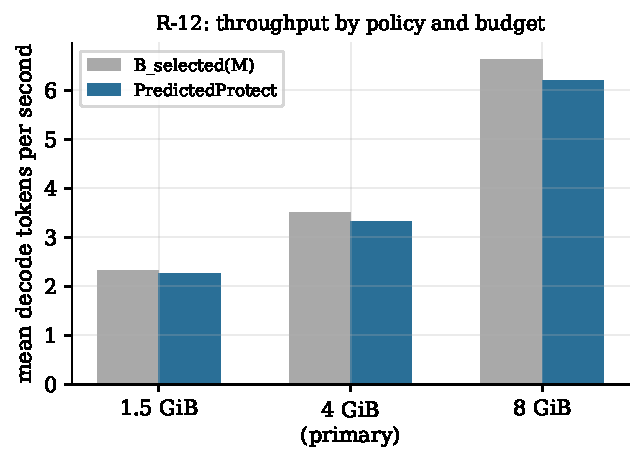
\includegraphics[width=0.78\linewidth]{figures/figure_c4_r2_12_throughput_by_budget.pdf}
\caption{R2-12: mean real-runtime decode tokens/second by policy and
budget. 4~GiB is the frozen primary endpoint; 1.5/8~GiB are secondary and
descriptive only.}
\label{fig:c4-r2-12-throughput}
\end{figure}

\begin{figure}[t]
\centering
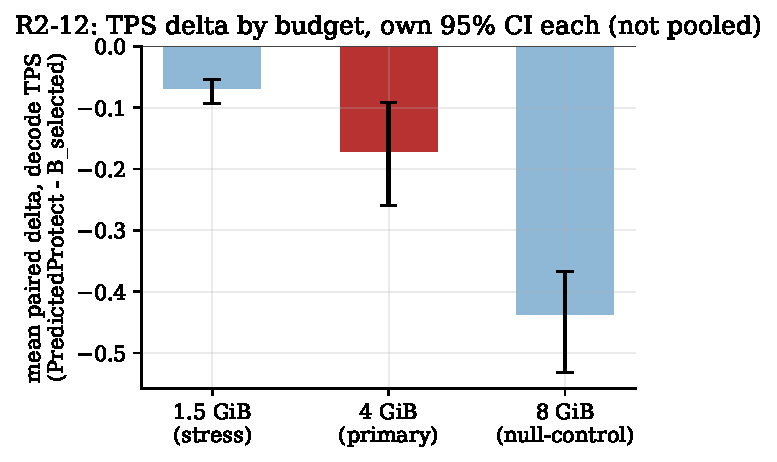
\includegraphics[width=0.78\linewidth]{figures/figure_c5_r2_12_delta_by_budget_ci.pdf}
\caption{R2-12: mean paired delta in decode tokens/second
(PredictedProtect $-$ B\_selected(M)) by budget, each with its own frozen
95\% paired bootstrap CI (not pooled across budgets). The primary 4~GiB
classification is \textsc{R2\_12\_FAIL}; 1.5/8~GiB are descriptive only and
do not carry an independent classification.}
\label{fig:c5-r2-12-delta}
\end{figure}

\subsection{Cross-Stage Synthesis}
\label{sec:iic-synthesis}

\begin{figure}[t]
\centering
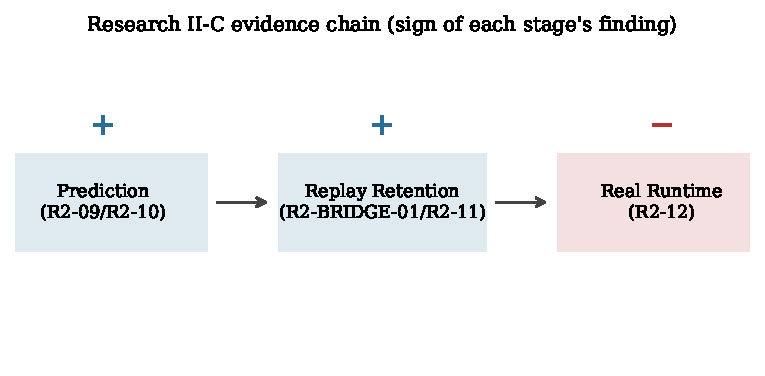
\includegraphics[width=0.78\linewidth]{figures/figure_c6_evidence_chain.pdf}
\caption{Research II-C evidence chain: prediction (positive) $\rightarrow$
replay retention (positive) $\rightarrow$ real runtime (negative). Each
stage measures a different quantity under a different experimental
apparatus; a negative result at one stage does not retroactively alter a
positive result at an earlier stage.}
\label{fig:c6-evidence-chain}
\end{figure}

\begin{center}
\begin{tabular}{@{}lll@{}}
\toprule
Level & Finding & Scope \\
\midrule
1. Prediction (R2-09/R2-10) & Positive (Category B; EVAL-confirmed margin) & Prediction quality only \\
2. Replay retention (R2-BRIDGE-01/R2-11) & Positive (\textsc{bridge\_positive}; \textsc{r2\_11\_pass}) & Replay miss-byte metric only \\
3. Real runtime (R2-12) & Negative (\textsc{r2\_12\_fail}) & Real decode throughput, primary budget \\
\bottomrule
\end{tabular}
\end{center}

These three findings are not in tension with one another: each measures a
different quantity, under a different (and progressively more realistic)
experimental apparatus, and none of the first two findings is invalidated by
the third. No predictor-quality or retention-improvement claim from R2-10,
R2-BRIDGE-01, or R2-11 is weakened, retracted, or reclassified merely
because real-runtime throughput failed to improve at R2-12.

The central conclusion of Research~II-C is accordingly conservative:
predictive expert information is measurably useful for forecasting routing
and can improve a replay-level retention metric, but the tested
\emph{reactive} predictive-retention realization -- one that only changes
which resident object is evicted on a miss, without changing when a fetch is
issued relative to ongoing computation -- does not convert that information
into improved end-to-end decode throughput on the evaluated runtime
configuration. Section~\ref{sec:iic-related-work} below situates this
result against systems in the literature that \emph{do} report throughput
gains from predictive expert handling.

\subsection{Related Work in Context}
\label{sec:iic-related-work}

A line of systems work on memory-constrained MoE inference reports measured
throughput or latency gains from combining expert-use prediction with an
\emph{active} mechanism for acting on that prediction before a miss reaches
the decode critical path: proactive prefetching with reordered inference
\cite{promoe2025}, joint prediction-plus-scheduling that explicitly
decouples I/O from computation \cite{prescope2025}, semantic-hint-driven
joint prefetch/cache/offload decisions \cite{finemoe2026}, predictive
caching paired with token scheduling \cite{expertflow2026}, data-aware
GPU-CPU hybrid prefetch/pre-calculation \cite{daop2025}, and speculative
pre-execution of likely-needed experts \cite{speculatingexperts2026}
(evaluated on the same Qwen3-30B-A3B model family used here)
\cite{moespeq2026}. Edge0 \cite{edge02026}, targeting the same
consumer-hardware, SSD-served deployment regime as this programme, predicts
the \emph{next} layer's routing one token ahead and stages the read during
the \emph{current} layer's computation, directly addressing the timing
constraint that a layer's expert set cannot be known before the previous
layer's output exists. Whether a given MoE model's routing is even
amenable to this class of techniques is itself an open question
\cite{localroutingconsistency2025}.

Every one of these systems pairs prediction with a mechanism that changes
\emph{when} a fetch is issued relative to compute. This programme's R2-12
realization tested only the narrower mechanism of changing \emph{which}
resident object is evicted on a reactive miss (\texttt{PredictedProtectPolicy}),
with no prefetch, scheduling, or compute/I/O overlap component. R2-12's
negative real-runtime result is consistent with this literature's implicit
premise -- that an active timing mechanism, not prediction alone, is what
converts predictive accuracy into measured throughput -- rather than being in
tension with it. This framing was available independent of, and is not a
retrofit to accommodate, the R2-12 outcome: the distinction between
retention (what is evicted) and prefetch/scheduling (when a fetch is issued)
is a property of the system designs being surveyed, not of Argine's result.
This programme does not claim priority or comparative superiority over any
of the cited systems; none was reimplemented or benchmarked head-to-head
against Argine's runtime.

\section{Conclusion (Provisional, II-A Only)}
\label{sec:conclusion}

This report establishes, under a behaviorally validated offline replay
model of a real 30B-A3B MoE coding-workload trace
(Section~\ref{sec:replay-validation}), that a substantial gap exists
between causal LRU-family expert retention and a non-causal Belady-optimal
upper bound, at every tested capacity-constrained expert-memory budget
(Sections~\ref{sec:oracle-headroom}--\ref{sec:sensitivity-capacity}). We
decompose this gap into a small, non-monotonically-signed structural
component attributable to the runtime's sharded retention architecture,
and a substantially larger policy-information headroom
(Section~\ref{sec:recoverable-envelope}) -- the scientifically clean
upper bound motivating future causal retention and prediction research.
The largest tested relative headroom occurs near $8$~GiB ($70.66\%$) and
the largest tested absolute headroom near $1.5$~GiB
($\approx 103.57$~GB); the gap collapses entirely once the working set
becomes effectively resident at $16$~GiB, the first tested such point.

This is a provisional conclusion, limited strictly to Research II-A. It
establishes an upper bound on recoverable retention performance; it does
not establish, estimate, or imply any demonstrated causal recoverability,
latency improvement, or production performance gain. Research II-B
(whether exploitable routing structure exists) and Research II-C
(whether a causal predictor can recover any of this headroom, and
validation against the real runtime) remain future work, not yet
started. The present II-A tranche is frozen as of the commit and run IDs
recorded in Appendix~\ref{sec:provenance-appendix} and
\texttt{II-A-FREEZE.json}, and is intended to be incorporated, without
silent strengthening of its claims, into the eventual combined
II-A+II-B+II-C Research Part 2 paper.


\appendix
\section{Provenance Appendix}
\label{sec:provenance-appendix}

\subsection{II-A canonical runs (preserved)}
\begin{table}[h]
\centering
\caption{Canonical run identity for the II-A tranche. The historical II-A
freeze record remains \texttt{II-A-FREEZE.json}.}
\label{tab:provenance-iia}
\small
\begin{tabular}{@{}llll@{}}
\toprule
Experiment & Run ID & Outcome & Git commit \\
\midrule
R2-01 & \texttt{bb6d8ca3\ldots} & PASS & \texttt{76baf459\ldots} \\
R2-02 & \texttt{238c8ee7\ldots} & PASS & \texttt{7a36083b\ldots} \\
R2-03 & \texttt{d9570770\ldots} & PASS & \texttt{0cdc657a\ldots} \\
R2-04 & \texttt{cd2b58b0\ldots} & PASS & \texttt{b6f0fd79\ldots} \\
\bottomrule
\end{tabular}
\end{table}

\noindent Validated source trace SHA-256 (II-A and R2-05--R2-07):
\texttt{e6c16f2bcdb4ef841770ff16ac404c91312297112bcd7e653438cc22b8d7b2f1}.

\subsection{II-B canonical runs}
\begin{table}[h]
\centering
\caption{Canonical run identity for the II-B tranche. See
\texttt{II-B-FREEZE.json} for the machine-readable manifest.}
\label{tab:provenance-iib}
\small
\begin{tabular}{@{}p{1.1cm}p{3.2cm}p{1.1cm}p{5.7cm}@{}}
\toprule
Exp. & Run ID & Outcome & Canonical digest (prefix) \\
\midrule
R2-05 & \texttt{da82e15b61c94019840477642618565a} & PASS & \texttt{4a1b72cdfcd37144\ldots} \\
R2-06 & \texttt{2e075161f02443ff822279add6938ca4} & PASS & \texttt{a727edf427352864\ldots} \\
R2-07 & \texttt{af28e8c6dc5044a18e4a86137d59156a} & PASS & \texttt{ad36e615970b196b\ldots} \\
R2-08 & \texttt{6165471a12574e05b48932aac2f1626c} & PASS & \texttt{f5db4e0bf43ce424\ldots} \\
\bottomrule
\end{tabular}
\end{table}

\noindent Full II-B canonical digests (from frozen manifests/summaries):
R2-05 \texttt{4a1b72cdfcd37144446fc1a106b6fa8d559d10bc0729e1baf16dda7c1fa620df};
R2-06 \texttt{a727edf42735286420d326baad481687167d3d0aba0444a527183c084140926e};
R2-07 \texttt{ad36e615970b196b64ba3a3fdc2559e252cc8627e5d17d0d830d16742f59281a};
R2-08 \texttt{f5db4e0bf43ce4243edb303441e82ceefa5a0aeb5754143292f1230f220527c3}.

\subsection{R2-08 controlled-capture provenance}
R2-08 canonical matrix: 4 workloads $\times$ 2 replicates = 8 valid cells,
matched decode horizon $H=388$, 8 temporal windows of length 48, 1 reused
capture and 7 new captures. All canonical cells report compatible
configuration fingerprints and consistent model/runtime identities:
model SHA-256 \texttt{a015794bfb1d69cb03dbb86b185fb2b9b339f757df5f8f9dd9ebdab8f6ed5d32};
runtime SHA-256 \texttt{a0063720ec4bb5d1ba3e4f7c0387dd1bc6a239b0ce038ba3d755351dab3f5cf3}.
Deterministic decoding protocol: temperature $=0.0$, top-$k=1$.

\paragraph{Capture-ID audit (required before freeze).}
The reused \texttt{coding-v1/seed-42} cell carries
\texttt{capture\_run\_id = bb6d8ca34dbc4537a43d54be30c9f3e1} and
\texttt{capture\_source = 286a41477ce54d5fb9ccc24f4e508f22} from R2-01.
The seven R2-08-managed new cells carry
\texttt{capture\_run\_id = null} and \texttt{capture\_source = null}, but
each has trace path, trace SHA-256, workload identity/version, seed,
model SHA-256, runtime SHA-256, configuration fingerprint, validation
state, canonical status, and is bound to the canonical R2-08 run and
digest. This is documented as an intentional provenance representation for
R2-08-internal captures under the R2-08 run identity; trace SHA and
canonical run identity are sufficient to identify the evidence. No capture
IDs were invented, no scientific traces were modified, and no model
capture was recaptured for the paper freeze.

\subsection{Freeze records}
The II-A historical freeze remains \texttt{II-A-FREEZE.json}. The II-B
freeze record is \texttt{II-B-FREEZE.json}. This cumulative
II-A+II-B+II-C manuscript is provisional; II-C remains future work.

{\small
\bibliographystyle{unsrt}
\bibliography{references}
}

\end{document}
